
\subsubsection{12.11.14} 

\begin{enumerate} 
	\item Время начала и окончания собрания:
	19:00 - 20:30
	\item Цели собрания:
	\begin{enumerate}
		\item Испытать программу раздельного управления роботом с двух джойстиков.
		
		\item Включить в программу управления роботом программу управления механизмом захвата корзины.
		
		\item Заменить шестеренки в механизме захвата корзины с больших на более компактные.
		
		\item Придумать, из каких материалов мы будем конструировать ковш для мячей.
		
	\end{enumerate}
	
	\item Проделанная работа:
	\begin{enumerate}
		\item Поскольку из-за больших шестеренок конструкция механизма захвата корзины занимала слишком много места, было решено заменить их на маленькие. Так как маленькие шестеренки у нас закончились, было решено снять с робота те две из них, которые использовались для крепления перекладины на подъемнике. Шестеренки были сняты и заменены на крепления, изготовленные из алюминиевого профиля.
		
		\begin{figure}[H]
			\begin{minipage}[h]{0.2\linewidth}
				\center  
			\end{minipage}
			\begin{minipage}[h]{0.6\linewidth}
				\center{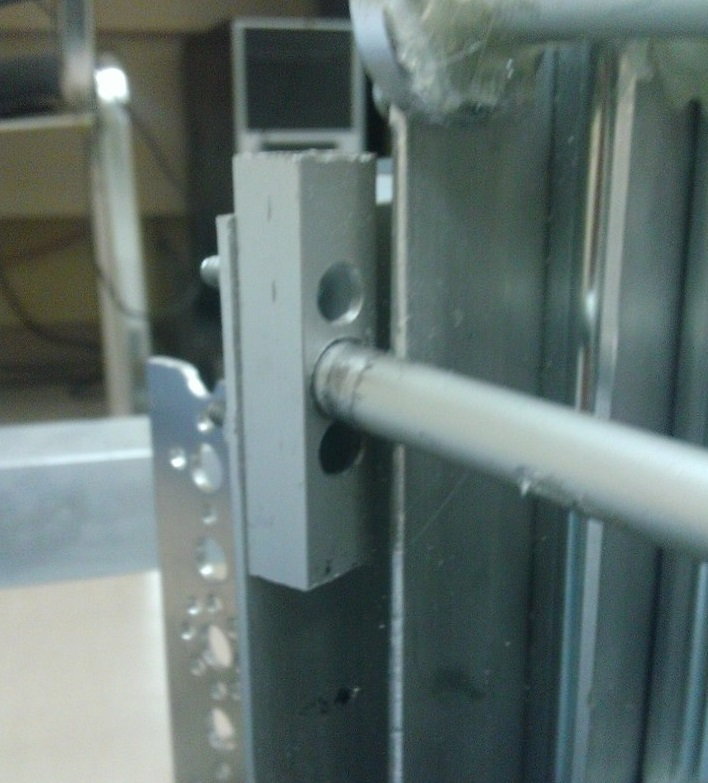
\includegraphics[scale=0.3]{days/12.11.14/images/01}}
				\caption{Крепление перекладины заменено}
			\end{minipage}
		\end{figure}
		
		\item Шестеренки в механизме захвата корзины заменены на более компактные.
		
	%	\begin{figure}[H]
	%		\begin{minipage}[h]{0.2\linewidth}
	%			\center  
	%		\end{minipage}
	%		\begin{minipage}[h]{0.6\linewidth}
	%			\center{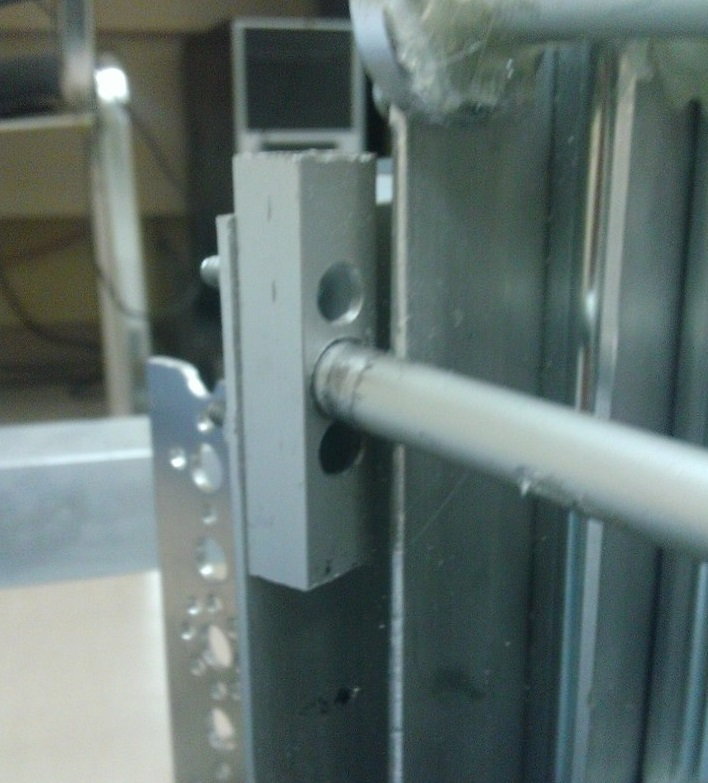
\includegraphics[scale=0.5]{days/12.11.14/images/01}}
	%			\caption{Замена шестеренок}
	%		\end{minipage}
	%	\end{figure}
		
		\item На общекомандном обсуждении было решено использловать для создания ковша для мячей Металлическую сетку с мелкими ячейками, поскольку она обладает достаточной жесткостью, но при этом легко сгибается. При этом, сетка обладает малой массой, что важно, поскольку она будет подниматься на 120 см. Кроме того, через ячейки сетки можно будет легко видеть, какое количество мячей находится в ковше.
		
		\item Программа управления механизмом прицепа не реализована.
		
		\item Программа раздельного управления роботом с двух джойстиков не была испытана.
		
	\end{enumerate}
	
	\item Итоги собрания:
	\begin{enumerate}
		\item Механизм прицепа доработан.
		
		\item Программа управления прицепом не реализована.
		
		\item Программа раздельного управления роботом не испытана.
		
	\end{enumerate}
	
	\item Задачи для последующих собраний:
	\begin{enumerate}
		\item Включить в программу управления роботом программу управления механизмом прицепа.
		
		\item Испытать программу раздельного управления роботом с двух джойстиков.
		
	\end{enumerate}     
\end{enumerate}
\fillpage

